% This template was originally by R. Jacob Vogelstein
% Updated on March 1, 2010 by Noah J. Cowan
% Updated on May 18, 2014 by Brian Weitzner
% at https://github.com/weitzner/jhu-thesis-template
% Updated on January 29, 2016 by John Muschelli
% at https://github.com/muschellij2/PhD_Thesis
% Updated on April 13, 2016 by Leonardo Collado Torres and
% available at https://github.com/lcolladotor/jhu-thesis-template.
% Forked by John Clayton in December, 2019
% JHU Formatting requirements of Sheridan Libraries may be found at:
% https://www.library.jhu.edu/library-services/
% electronic-theses-dissertations/formatting-requirements/

% The document is based on the standard 12pt LaTeX report class
%\documentclass[12pt,draft]{report}
\documentclass[12pt]{report}

% PDF Creation settings
\pdfcompresslevel=9
\pdfminorversion=5
\pdfobjcompresslevel=2

% Needed to create a PDF/A file
\usepackage[a-1b]{pdfx}

% Incude pdf docs
\usepackage{pdfpages}
% For transferring hyperlinks from PDFs added by pdfpages
\usepackage{pax}

% For dialect-specific hyphenation etc.
\usepackage[american]{babel}

% T1 font encoding
\usepackage[T1]{fontenc}
% Use UTF8 input encoding
\usepackage[utf8]{inputenc}
%\DeclareUnicodeCharacter{00A0}{ }

% Load latin modern, a font with all the characters
\usepackage{lmodern}

% For generating the dummy text in the mwe template
\usepackage{lipsum}

% Provides various text symbols (such as \textdegree) in TS1 encoding.
\usepackage{textcomp}
\usepackage{amsmath}
\usepackage{amsfonts}
\usepackage{amsthm}
\usepackage{commath}

% provides ul for cv
\usepackage{soul}

% Set the margins according to JHU specifications
\usepackage{geometry}
 \geometry{
   letterpaper,
   left=1.5in,
   right=1.0in,
   top=1.0in,
   bottom=1.0in}

% Spacing options
\usepackage{setspace}

% Typography and fonts
\usepackage[protrusion]{microtype}
% For multiple columns
\usepackage{multicol}
% for proper text wrapping of nucleic acid sequences
\usepackage{seqsplit}

% Fancy verbatim-like environment for code
\usepackage{listings}
\lstset{basicstyle=\footnotesize\ttfamily,
        columns=flexible,
        breaklines=true
}

% Hyperlink handling
\usepackage[pdfa]{hyperref}
\hypersetup{
   linktocpage,
   unicode,
   colorlinks=true,
   citecolor=link,
   filecolor=link,
   linkcolor=link,
   urlcolor=link
}

% Color handling
\usepackage{xcolor}
%\usepackage{color}

% Color for links
\definecolor{link}{rgb}{0.45,0.51,0.67}

%%% Table of Contents %%%
\usepackage[titles]{tocloft}
% Dots for chapters too
\renewcommand{\cftchapleader}{\cftdotfill{\cftdotsep}}

% To add bibliography to the table of contents
\usepackage{tocbibind}

% Set depth of TOC items
\setcounter{tocdepth}{4}

% Set depth of section numbering
\setcounter{secnumdepth}{4}

\usepackage{calc}
% Tweak to TOC to add 'chapter' to chapter name instead of a number only
\renewcommand{\cftchappresnum}{\chaptername\space}
% Set width of box based on longest label name
\setlength{\cftchapnumwidth}{\widthof{\textbf{Appendix~II~}}}

% Stylize chapter headings
%\usepackage{sectsty}
%\chapterfont{\centering}

% Removes 'Chapter #' title while keeping
% it listed in the TOC
\newcommand\chap[1]{%
  \chapter*{#1}%
  \addcontentsline{toc}{chapter}{#1}}

% Removes 'Section #' title while keeping
% it listed in the TOC
\newcommand\sect[1]{%
  \section*{#1}%
  \addcontentsline{toc}{section}{#1}}

% Removes 'Subsection #'title while keeping
% it listed in the TOC
\newcommand\subsect[1]{%
  \subsection*{#1}%
  \addcontentsline{toc}{subsection}{#1}}

% For oligo table
% Changes dot to hyphen in figure references and captions
\renewcommand{\thetable}{\thechapter-\Roman{table}}
\usepackage{booktabs}
\usepackage{multirow}
\usepackage{longtable}
\usepackage{array}
\usepackage{pdflscape}

% Align on numeric decimal in table
%\usepackage{dcolumn}

% Enhanced control over layout of itemize, enumerate, and description
\usepackage{enumitem}

% Graphics Packages
%\usepackage{graphics} 
\usepackage{graphicx}
%\usepackage{float}

% Setup style for figure captions
\usepackage[font=small,
            labelfont=bf,
            labelsep=period,
            font=sf,
            hypcap=true]{caption}

% For captions on the side of figures
\usepackage{ifthen}
\usepackage[rightcaption]{sidecap}

% Individual panel captions
%\usepackage{subfig}

% Options for hyperlinking to floats
\usepackage[all]{hypcap}

% Graphics Path
\graphicspath{{../images/}}

% To change the name of the figures page
\renewcommand{\listfigurename}{Figures}
% To change the default beginning to each line
\renewcommand{\cftfigpresnum}{\bfseries Figure }
% Changes dot to hyphen in figure references and captions
\renewcommand{\thefigure}{\thechapter-\arabic{figure}}
% To change the distance to the start of the figure title
\setlength{\cftfignumwidth}{\widthof{\textbf{Figure~5-10~}}}

% Tikz, for drawing vector graphics
%\usepackage{tikz}
%\usetikzlibrary{positioning}
%\usetikzlibrary{shapes,arrows}

% Enable the glossary
%\makeglossary

% Make appendices
%\usepackage[title,titletoc]{appendix}
\usepackage{appendix}
%\renewcommand{\appendixname}{Appendix}

%%%%%%%%%%%%%%%%%%
% FOR BIBTEX
%%%%%%%%%%%%%%%%%%

% For use with IEEEtran.bst
%\usepackage{cite}
%\usepackage[numbers,square,compress]{natbib}
%\setlength\bibsep{4pt}
% Set bibliography name
%\usepackage{chbibref}
%\renewcommand\bibname{References}

%%%%%%%%%%%%%%%%%%
% FOR BIBLATEX
%%%%%%%%%%%%%%%%%%

\usepackage[
style = nature, 
sorting = none, 
%dashed = false,
%maxbibnames = 99,
backend = biber,
url=false,
isbn=false,
natbib = true
]{biblatex}

% Point to bibfile
\addbibresource{bibtex.bib}

% If you want to exclude some portions from the bibliography
%\AtEveryBibitem{
%\clearfield{issn}
%\clearfield{note}
%\clearfield{month}
%}

% Change bib font size
\renewcommand{\bibfont}{\small}

%%%%%%%%%%%%%%%%%%
% DOI from Segmentation (needs hyperref)
%%%%%%%%%%%%%%%%%%

%\makeatletter
%\providecommand{\doi}[1]{%
%  \begingroup
%    \let\bibinfo\@secondoftwo
%    \urlstyle{rm}%
%    \href{http://dx.doi.org/#1}{%
%      doi:\discretionary{}{}{}%
%      \nolinkurl{#1}%
%    }%
%  \endgroup
%}
%\makeatother

% Math
\usepackage{amsmath,amssymb,array}

\newtheorem{theorem}{Theorem}[section]
\newtheorem{corollary}{Corollary}[theorem]
\newtheorem{lemma}[theorem]{lemma}

%\newcommand{\bm}[1]{ \mbox{\boldmath $ #1 $} }
%\newcommand{\bin}[2]{\left(\begin{array}{@{}c@{}} #1 \\ #2
%             \end{array}\right) }
% A math shortcut frequently used by John Muschelli
%\newcommand{\bbeta}{\mbox{\boldmath $\beta$}}

%%%%%%%%%%%
% CONTENT %
%%%%%%%%%%%
%
\begin{document}
% Sets paragraph (and not title) spacing, roughly speaking
\setlength{\parskip}{3pt}
\baselineskip=24pt
%
% front matter page numbering
\pagenumbering{roman}
%
% Add title page
% JHU Dissertation title page
\thispagestyle{empty}
% baselineskip of 18pts (i.e. 1.5x spacing or 0.25")
% with 12pt type; 72 points per inch
\baselineskip=18pt
\begin{center}
% Spacer at top of page
\vspace*{3\baselineskip}
%
% TITLE GOES HERE
{\bfseries Malicious Network Traffic Detection via Deep Learning: \\An Information Theoretic View}\\[6\baselineskip]
%
by\\
%
% AUTHOR GOES HERE
Erick Galinkin\\[3\baselineskip]
%
%
A thesis submitted to The Johns Hopkins University in conformity\\
with the requirements for the degree of \\
Master of Science in Applied and Computational Mathematics\\[4\baselineskip]
%
Baltimore, Maryland\\
% DATE OF SUBMISSION HERE
June, 2020\\[6\baselineskip]
%
% UPDATE THE YEAR HERE
{\copyright{} 2020 E.~Galinkin\\
All rights reserved}
%
\end{center}
%
% Reset baseline skip to previous value
\baselineskip=24pt
\newpage 

%
% Setup and add front matter
\pagestyle{plain}
\setcounter{page}{2}
%
% Add abstract
\chapter*{Abstract}
%
The attention that deep learning has garnered from the academic community and industry continues to grow year over year, and it has been said that we are in a new golden age of artificial intelligence research.
However, neural networks are still often seen as a ``black box'' where learning occurs but cannot be understood in a formal way.
Using information geometry, we explore how homeomorphism affects the manifold on which learning occurs and the invariance of the mutual information captured by the coordinate system on that manifold under homeomorphism.
We empirically validate these results, using accuracy as a measure of similarity of learned representations.

Our results suggest that although the details of learned representations and the specific coordinate system defined over the manifold of all parameters differ slightly, the functional approximations are the same.
Furthermore, our results show that since mutual information remains invariant under homeomorphism, only feature engineering methods which alter the entropy of the dataset will change the outcome of the neural network.
Additionally, we show that for some datasets and tasks, neural networks require meaningful, human-driven feature engineering or changes in architecture to provide enough information for the neural network to generate a sufficient statistic.
Applying our results can serve to guide analysis methods for machine learning engineers and suggests that neural networks which can exploit the convolution theorem are equally accurate as standard convolutional neural networks, and can be more computationally efficient.
%
% Add Thesis Readers
\section*{Thesis Readers}
\begin{singlespace}
%
\noindent Dr.~Cleon Davis (Primary Advisor)\\
\indent \indent Senior Professional Staff\\
\indent \indent Johns Hopkins University Applied Physics Laboratory\\

\indent \indent and\\

\indent \indent Program Vice Chair Electrical and Computer Engineering\\
\indent \indent Lecturer and Research Faculty in Applied and Computational Mathematics\\
\indent \indent Johns Hopkins Engineering for Professionals\\


\noindent Dr.~Lanier Watkins\\
\indent \indent Program Chair\\
\indent \indent Department of Computer Science and Cybersecurity\\
\indent \indent Johns Hopkins University\\
\end{singlespace}
%
% Add readers (JHU style is to include readers with in abstract)
%\include{text/03-committee}
%
% Add preface
%\include{text/04-preface}
%
% Add dedication
% Adds a spacer where the header would be
\chapter*{~}
\addcontentsline{toc}{chapter}{Dedication}

\begin{center}
Y'all ain't ready - fuckin haters.
\end{center}

%
% Add acknowledgements
\chap{Acknowledgements}
%\addcontentsline{toc}{chapter}{Acknowledgements}

% INSERT TEXT HERE
I would like to extend my deepest gratitude to my thesis adviser, Cleon Davis, and my co-adviser Lanier Watkins.
I have learned so much in this process and you both have been incredibly supportive. 
No matter how far out over my skis I got, they found a way to pull me back in.
I hope that in the future, I will make you both proud to call me a peer.

I would also like to extend my gratitude to both Dr. Raymond Canzanese of Netskope, who was my work supervisor during much of my time at Johns Hopkins and Mr. Derek Abdine, who is my current work supervisor and was my supervisor during the writing of this thesis.
You have both always been patient, understanding, and flexible.
Without the two of you, I would likely not be continuing on in academia after this thesis, and I will forever be in your debt.

I would like to extend my gratitude to my colleague and friend Stella Biderman for all the time she spent hearing my crazy ideas and helping me contextualize them.

Lastly, my thanks to my dearest friends Dave and Emilee; the entire Rupeethon crew (Jon, Rich, Conor, Lynn, Scott, Steve); and my friends in the DEF CON AI village (Ariel, Rich, Sven, Yaga). 
No matter how galaxy-brained I got, you always listened and kept me inspired.
%
% To change the name of the contents page
%\renewcommand{\contentsname}{Contents}
%
% Create table of contents
\tableofcontents
%
% Create table list
%\listoftables
%
% Create List of figures
\listoffigures
\clearpage
%
%%% END FRONT MATTER %%%
%
%%%%% MAIN MATTER %%%%%
% Switch page numbering at the end of front matter, before first chapter
\pagenumbering{arabic}
%
%\begin{refsection}[myrefs.bib]
\chapter{Introduction}
\label{chap:intro}

\sect{\lipsum*[1][1]}

\subsect{\lipsum*[1][2]}

\lipsum[1-3]\parencite{darwin,newton,mendel}

% Figure 1-1
\begin{figure}[t] %  figure placement: here, top, bottom, or page
   \centering
%   
\includegraphics[width=\textwidth,height=\textheight,keepaspectratio]{fig_1-1}
   
\includegraphics[scale=1]{fig_1-1}
   \caption[{\lipsum*[1][1]}]{\lipsum*[1][1-2]}
   \label{fig:fig_1-1}
\end{figure}

\subsect{\lipsum*[1][3]}

\lipsum[4-7]\parencite{malthus,einstein,nash}

% Figure 1-2
\begin{figure}[p] %  figure placement: here, top, bottom, or page
   \centering
%   
\includegraphics[width=0.50\textwidth,height=\textheight,keepaspectratio]{fig_1-2}
   
\includegraphics[scale=1]{fig_1-2}
   \caption[{\lipsum*[1][2]}]{\lipsum*[1][2-6]}
   \label{fig:fig_1-2}
\end{figure}

\subsect{\lipsum*[1][4]}

\lipsum[7-10]\parencite{constable,hardy}

\subsect{\lipsum*[1][5]}

\lipsum[12-13]\parencite{morgan,sturtevant,fisher}

% Figure 1-3
\begin{figure}[tb] %  figure placement: here, top, bottom, or page
   \centering
%   
\includegraphics[width=\textwidth,height=\textheight,keepaspectratio]{fig_1-3}
   
\includegraphics[scale=1]{fig_1-3}
   \caption[{\lipsum*[1][3]}]{\lipsum*[1][3-7]}
   \label{fig:fig_1-3}
\end{figure}

\subsect{\lipsum*[1][6]}

\lipsum[16-20]\parencite{dobzhansky,nietzsche}

% New section
\sect{\lipsum*[2][1]}

\subsect{\lipsum*[2][1]}

\lipsum[23-26]\parencite{weber}

\subsect{\lipsum*[2][2]}

\lipsum[27-30]\parencite{hershey,feynman}

% Figure 1-4
\begin{figure}[p] %  figure placement: here, top, bottom, or page
   \centering
%   
\includegraphics[width=\textwidth,height=\textheight,keepaspectratio]{fig_1-4}
   
\includegraphics[scale=1]{fig_1-4}
   \caption[{\lipsum*[1][4]}]{\lipsum*[2][4-8]}
   \label{fig:fig_1-4}
\end{figure}

\lipsum[31-34]\parencite{watson,hawking}

\subsect{\lipsum*[2][3]}

\lipsum[35-42]

\subsect{\lipsum*[2][4]}

\lipsum[43-45]

% New section
\sect{\lipsum*[3][1]}
\label{sect:one-three}

\subsect{\lipsum*[3][2]}

\lipsum[47-49]

\subsect{\lipsum*[3][3]}
\label{subsect:one-three-two}

\lipsum[51-52]

\subsect{\lipsum*[3][4]}

\lipsum[53-55]

% New section
\sect{\lipsum*[4][1]}

\lipsum[57-58]
%\printbibliography[title=References]}
%\end{refsection}
%
%\begin{refsection}[myrefs.bib]
\include{text/08-chapter2-preliminaries}
%\printbibliography[title={References}]
%\end{refsection}
%
%\begin{refsection}[myrefs.bib]
\chapter{Experiment 1 - Dataset and in-Network Transformation of MNIST}
\label{chap:five}

\section{Motivation}
In order to contextualize the results of the experiments we wish to conduct on malware data, we consider the methods presented there on the well-studied MNIST Database of Handwritten Digits~\cite{lecun1998mnist}.
MNIST is a benchmark in computer vision - since our baseline convolutional neural network is based on LeNet~\cite{lecun1998gradient}, we have a large body of research to compare to.
Additionally, MNIST serves as an introduction to the field of computer vision for many students and so our architectures and theories can be made more accessible in that context.
The current state of the art for MNIST~\cite{byerly2020branching}, achieved in January of this year achieves a 99.84\% accuracy.
The best results achieved in the original LeCun paper was 99.3\% accuracy and generally an accuracy greater than 98\% is considered to be good.

\section{Methodology}
In order to maintain consistency with our other findings, our methodology is identical to experiments in \ref{chap:three} and \ref{chap:four}, leveraging the same hardware as in \ref{append:one} and the same model details as in \ref{append:two}.
In this case, our dataset differs from our previous two experiments by virtue of being a ``true'' image dataset. 
As a result, some preprocessing work was required to reshape our 32 x 32 images into a flat vector, this is done without loss of information.

\section{models}
All code\footnote{Code is available at the following url: \url{https://github.com/erickgalinkin/jhu_masters}} was written in Python, using the Tensorflow 2, PyTorch, and Scikit-learn libraries.
Only the baseline models described in \ref{other models} used the Scikit-learn library, and only the Wavelet Convolutional network described in \ref{wavelet cnn} used PyTorch.
The remaining models all used the Tensorflow framework.

\subsection{Fully-Connected Neural Network}
The fully-connected neural network architecture accepts, as input, a 1x100 row-vector.
This vector is then fed to three densely connected layers, each with 256 ReLU-activated neurons.
The output neuron is a single sigmoid-activated neuron, which provides a probability of traffic being benign.

\subsection{Standard Convolutional Neural Network}
Our standard convolutional neural network is a sequential model which accepts the same sort of input as our fully-connected neural network, and passes it to an architecture comprised of two convolution and max-pooling blocks, followed by batch normalization, and then passed to two densely connected layers of 128 neurons each. The architecture is visualized below in figure \ref{fig:conv net}.

\begin{figure}[ht]
\caption{Convolutional Neural Network Architecture}
\label{fig:conv net}
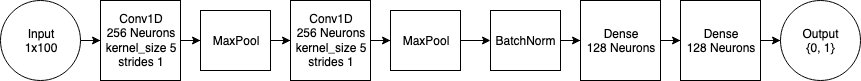
\includegraphics[width=\textwidth]{conv_architecture}
\centering
\end{figure}

\subsection{Other Models} \label{other models}
Two baseline models were considered.
The first is the random forest model provided in the Scikit-learn library with no hyperparameter tuning.
Decision tree models are generally good at classification tasks~\cite{hastie01statisticallearning} but are weak classifiers which are sensitive to variance.
Random forests are a the result of averaging a large collection of de-correlated trees and provide a good benchmark as a na\"ive model - in the respect that it is untuned - for classification.

The other benchmark model is a Support Vector Classifier, again provided by the Scikit-learn library.
The rationale for using a Support Vector Machine is that we wanted to see if some hyperplane could be learned which would separate the data.
This model was again, na\"ive in the respect that it was merely the ``out of the box'' model, and so the classifier was built on top of the radial basis function kernel.

\section{Results}

\begin{table}[h]
\caption{Neural Network Results}
\centering
\label{Tab:test}	
\begin{tabular}{l|ll}
\textbf{Data and Architecture}  & \textbf{Test Accuracy} & \textbf{Mean Step Time} ($\mu$s) \\\cline{1-3}
Raw, Fully-Connected NN            & 97.73\%         & 29\\
Fourier, Fully-Connected NN        & 98.12\%         & 41\\
Wavelet, Fully-Connected NN        & 97.83\%         & 30\\
\hline
Raw, Convolutional NN              & 99.11\%         & 204\\ 
Fourier, Convolutional NN          & 99.10\%         & 237\\
Wavelet, Convolutional NN          & 99.10\%         & 212\\
\hline
Raw, Fourier NN                    & 98.45\%         & 959\\
Raw, Wavelet NN                    & 98.89\%         & 1068\\ 
\end{tabular}
\end{table}

In this case, all of our models achieve accuracy over 97\% which is broadly considered to be the benchmark accuracy for MNIST. 
For all these combinations of architecture and transformation, the difference between our maximum accuracy score of 99.11\% and our minimum accuracy of 97.73\% is only 1.38\%.
Comparing the convolutional models in particular, the difference between the Raw, Fourier-transformed, and Wavelet-transformed data is only 0.01\%. 
%\printbibliography[title={References}]
%\end{refsection}
%
%\begin{refsection}[myrefs.bib]
\chapter{Experiment 2 - In-Network Malware Dataset Transformation}
\label{chap:four}


\sect{Malware Classifier} \label{malware classifier}
As shown in Table~\ref{Tab:test}, the Random forest classifier outperforms all of the neural network and support vector machine architectures.
It is also noteworthy that the Fourier-transformed data fed to the convolutional Neural Network appears to misclassify an extremely high percentage of samples, and by flipping the labels on the test samples, we actually achieve 72.6\% accuracy, making it our second most accurate neural network classifier.

 
\begin{table}[ht]
\caption{Android App Data Test Results}
\centering
\label{Tab:test}	
\begin{tabular}{lll}
Data and Architecture Combination & Test Accuracy & mean step time (ms) \\
Raw, Fully-Connected NN           & 62.60\%         & 13\\
Raw, Convolutional NN             & 72.89\%         & 54\\
Fourier, Fully-Connected NN       & 58.88\%         & 12\\
Fourier, Convolutional NN         & 70.81\%         & 56\\
Wavelet, Fully-Connected NN       & 61.95\%         & 12\\
Wavelet, Convolutional NN         & 70.77\%         & 52\\
Raw, Fourier NN                   & 66.59\%         & 553\\
Raw, Wavelet NN                   & 73.33\%         & 623\\
Raw, Random Forest                & 79.80\%         & N/A\\
Raw, Support Vector Classifier    & 55.28\%         & N/A           
\end{tabular}
\end{table}

%\printbibliography[title={References}]
%\end{refsection}
%
%\begin{refsection}[myrefs.bib]
\chapter{Experiment 3 - In-Network Malware Dataset Transformation}
\label{chap:four}

In this experiment, we consider the work of Pratt~\cite{pratt2017fcnn} and Fujieda~\cite{fujieda2017wavelet} under the mutual information theory.
Both the Fourier and Wavelet neural networks take advantage of the convolution theorem - that is, given two functions $f$ and $g$,
\begin{align}
(f * g)(t) & = \int_{-\infty}^{\infty} f(\tau)g(t-\tau)dt \\
& = \int_{\mathbb{R}^n}f(x) e^{-2\pi i x \nu} dx	 \cdot \int_{\mathbb{R}^n}g(x) e^{-2\pi i x \nu} dx\\	
& = \mathcal{F}\{f\}(\nu) \cdot \mathcal{F}\{g\}(\nu)
\end{align}

and in the inverse, we get:
$$f \cdot g = \mathcal{F}^{-1}\{\mathcal{F}\{f\} * \mathcal{F}\{g\}\}$$

This allows us to avoid the high computational cost of performing a convolution via the sliding-tile method and instead potentially take advantage of the convolution theorem to perform convolution at the speed of the dot product.

\section{Methodology}
In this experiment, we use the same raw dataset, fully-connected neural network, and convolutional neural network as before, and we report the results of the ``control group'', the support vector classifier and random forest.
The results of these experiments are verbatim from \ref{chap:three}.
We also introduce two additional models to evaluate the effect of transformation on the learned representations.
The Fourier network and wavelet network differ from a conventional convolutional neural network by performing an in-layer transformation before the activation function is applied. 
Other than this difference in how the convolution is performed, the architecture of the Fourier network is identical to our convolutional network, and our wavelet network removes the pooling layers for reasons explained along with other architecture details in \ref{append:two}.


\subsection{Fourier Convolutional Neural Network}
Our Fourier ``Convolutional'' neural network is identical architecturally to our standard convolutional neural network, only with the convolutional layers replaced by Fourier layers.
Here, we put the word convolutional in quotes due to the fact that no actual convolution is performed.
To be more intellectually honest, we should refer to this network instead as a ``Fourier Transform Cross Product Network'', though this may confuse readers unfamiliar with the relationship.
In the interest of broad understanding, the term convolutional neural network is used when it helps clarify meaning even in spite of being a slight misnomer.

Specifically, the Fourier Convolutional Neural Network leverages a custom Fourier layer, which moves the data into Fourier space via the Fast Fourier Transform and then multiplies the transpose of the weight matrix with the input to the matrix.
Specifically, given an input $X^{(n)}$ and an output $A$, where the superscript is not an exponent, but instead indicates the layer of the input, the Fourier layer, $\ell$ acts on $X$:
\begin{align*}
X^{(n+1)} & = a \\
& = \ell^{(n)}(X^{(n)}) \\
& = \sigma(\mathcal{F}^{-1}(\mathcal{F}(X^{(n)})\cdot \mathbf{W}^{(n)\top}))
\end{align*}
Where $\mathcal{F}$ is the Fast Fourier Transform, $\sigma$ is the activation function - ReLU in this case - and $\mathbf{W}$ is the weight matrix for layer n.

\subsection{Wavelet Convolutional Neural Network} \label{wavelet cnn}
The network is constructed to accept a 100-dimensional row vector as input.
This input is then sent to the "wavelet layer" where it undergoes a Daubechies discrete wavelet transform.
The output is cast to a tensor which is multiplied against the transpose of the weight tensor.
This output then undergoes an inverse discrete wavelet transform with respect to the same mother wavelet.
As a result, the output of the layer remains the same shape as the input to the layer and so this architecture differs slightly from the other networks, since we do not use max pooling. 
The effect of this change to the architecture is not significant enough to be noteworthy.

The Wavelet Convolutional Neural Network implements similar functionality to our Fourier Neural Network, using the Continuous Wavelet Transform in lieu of the Fourier transform.
Due to the fact that there is a time component and a frequency component, the wavelet neural network has a different in-layer dimensionality than our other models, but is otherwise architecturally nearly identical.
These models were trained and evaluated on the same hardware as in \ref{chap:three}, with details in \ref{append:one}.
As before, the model accuracy was recorded over 100 trials and the average accuracy and average mean step time are reported.

\section{Results}
\begin{table}[ht]
\caption{Neural Network Results}
\centering
\label{Tab:test}	
\begin{tabular}{l|ll}
\textbf{Architecture}  & \textbf{Test Accuracy} & \textbf{Mean Step Time} ($\mu$s) \\\cline{1-3}
Fully-Connected NN            & 63.40\%         & 13\\
Convolutional NN              & 72.89\%         & 54\\  
Fourier NN                    & 63.27\%         & 143\\
Wavelet NN                    & 74.85\%         & 228\\
Random Forest                 & 80.28\%         & N/A\\ 
Support Vector Classifier     & 65.77\%         & N/A       
\end{tabular}
\end{table}

Again, the random forest outperforms all of our other classifiers.
It is worth noting that one of the primary motivations for replacing the sliding-tile convolution method with a Fourier or Wavelet method is the performance.
However, as we observe, the Fourier and Wavelet networks are significantly slower than their untransformed counterparts.
We conclude that the computational overhead of performing a transform and its corresponding inverse transform outweighs the speed-up gained by eliminating the sliding-tile convolution on smaller datasets, and the method as demonstrated in Pratt~\cite{pratt2017fcnn} should be reserved for relatively large images, where convolution is extremely slow.
In our case, we see a 2.65x increase in step time between a standard convolution and the Fourier method. 
Unfortunately, our activation functions do not behave nicely in the Fourier or Wavelet domain, as they operate linearly with respect to the space. 
The question of using a novel convolution operator and conducting the activation in that space has been addressed by Chakraborty~\cite{chakraborty2019surreal} but goes well beyond the question of simply adapting an activation function to the Fourier or Wavelet space.
The search for a "spectral activation" function is still an open question.
%\printbibliography[title={References}]
%\end{refsection}
%
%\begin{refsection}[myrefs.bib]
\chapter{Conclusions and Further Work}
\label{chap:conclusion}

\section{Malware data experiments}
Across both experiments, no neural network was able to match the performance of the 


\section{What a Neural Network Learns}
The preceding sections suggest that the representation learned by the neural network, $\hat{X}$ constitutes a minimum sufficient statistic of $X$. 
Moreover, that the mutual information satisfied the data processing inequality with respect to the Markov chain $Y \to X \to \hat{X}$: $I(Y; X) \geq I(Y; \hat{X})$.
Additionally, the invariance of mutual information under homeomorphism suggests that any smooth, uniquely invertible map on $X$ does not impact the learned representation and that instead only methods of feature extraction~\cite{goodfellow2016deep} which change the data in ways that meaningfully change the entropy of $X$ are useful.
This reinforces the idea~\cite{goodfellow2014explaining} that probability mass is concentrated in locally-connected regions approximated by small manifolds with significantly lower dimensionality than $X$ itself.
%\printbibliography[title={References}]
%\end{refsection}
%
%%%%% BACK MATTER %%%%%
%
%%% BIBLATEX BIBLIOGRAPHY %%%
%\footnotesize
\printbibliography[title={References},heading=bibintoc]
%
%%% BIBTEX BIBLIOGRAPHY %%%
%
% Use the IEEEtran.bst style file (bibtex)
%\bibliographystyle{IEEEtran}
%
% Name the bibliography
%\setbibref{References}
% Point to bibfile
%\footnotesize\bibliography{IEEEabrv,classics}
%\bibliography{IEEEabrv,classics}
%
% APPENDICES
\begin{appendices}
% Appendix I
%\thispagestyle{empty}
\footnotesize
% Setup and stylize appendices to integrate with TOC
\addtocontents{toc}{\protect\renewcommand\protect\cftchappresnum{\appendixname~}}
\renewcommand{\thechapter}{\Roman{chapter}}

% Stylize section header
\renewcommand{\thesection}{\Alph{section}.}

\chapter{Hardware}
\label{append:one}

All models were trained on the same hardware with the following specifications:

\quad\textbf{CPU}: AMD Ryzen Threadripper 2920x 12-core 3.5 GHz

\quad\textbf{RAM}: 128 GB 3200 MHz DDR4

\quad\textbf{GPU}: Nvidia RTX 2080 Ti 12GB

All models for which the software was compatible with GPU were trained on GPU.
Datasets were all small enough to be held in memory after having been read from disk so disk i/o latency was not a factor in training times.
\end{appendices}
%
%%% Biographical Sketch %%%
\chap{Biographical sketch}
% Reset the default paragraph style
\normalsize
\nonfrenchspacing
\doublespacing
\setlength{\parindent}{15pt} % default value for 12pt report
\setlength{\parskip}{3pt} % document default

% BIOSKETCH TEXT HERE
Erick Galinkin was born in Port Jefferson, New York.
After graduating from Miller Place High School in 2007, he spent a brief time at Stony Brook University where he studied Chemistry. 
In 2008, he joined the United States Air Force as a Chinese Language Analyst and spent 6 years enlisted, separating as a Staff Sergeant.
During his time in the Air Force, Erick obtained an Associate's Degree in Mandarin Chinese from the Defense Language Institute and a Bachelor's Degree in Cybersecurity from the University of Maryland Global Campus.
In 2014, Erick began working as a Research Engineer for Cisco Systems and shortly thereafter began pursuing a masters in information assurance, also from University of Maryland Global Campus, graduating in 2017.
Erick has also obtained a graduate certificate in bioinformatics from UMGC, and worked as a Senior DevOps Engineer at Optiv prior to starting at Johns Hopkins.
Beginning in September 2018, Erick enrolled at Johns Hopkins while working as a Security Research Scientist at Netskope. 
In January, 2020 he began work as a Principal AI Researcher at Rapid7.
Presently, Erick has accepted an offer to further his studies as a PhD student in Computer Science at Drexel University.
%
\end{document}